\chapter{Medical Fundamentals}
Comprehension of the physiological functionality of the human heart and the cardiovascular system is an important prerequisite to the work addressed in this thesis. Therefore the basics of these topics will be explained in this chapter.

\section{Cardiovascular System}
The fundamental task of the cardiovascular system is to supply all organs with blood. The system, is divided into two components. The systemic circulation and the pulmonary circulation. As shown in Figure \ref{fig:circulation}, which represents the percentage distribution of the blood over the circulatory system, the systemic circulation is supplying blood flow to all tissues and organs except the lung. Due to this it is also referred to as the greater circulation. \cite{GH20} The center of the circulatory system is the heart. The heart itself consists of two mechanical pumps, which are functionally connected in series, but are united in one organ \cite{HKS4}. It is seperated into two sides, which themselfs are divided into an atrium and a ventricle.  \cite{HKS7} Through contraction the heart is pumping blood into the circulatory system. 

\begin{figure}
  \centering
  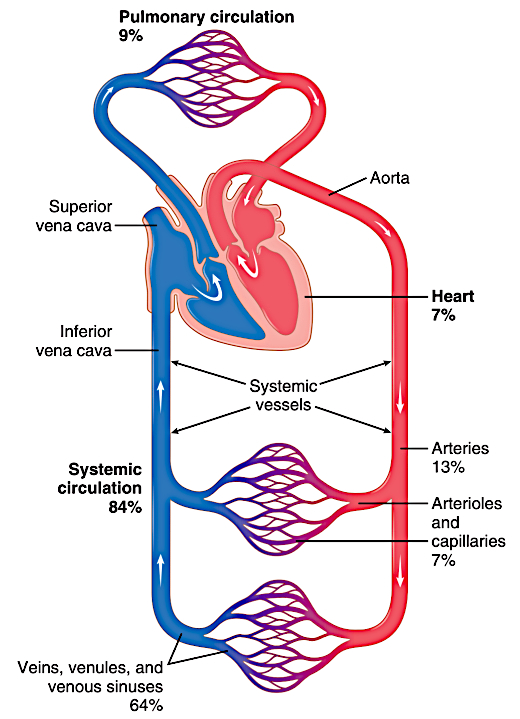
\includegraphics[width=0.4\textwidth, height=0.6\textwidth]{images/circulation.jpg}
  \caption{Blood distribution in circulatory system \cite{GH20}}
  \label{fig:circulation}
\end{figure}

\begin{figure}[h]
  \centering
  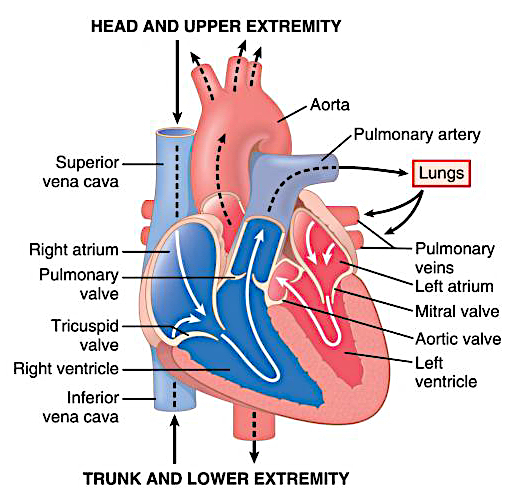
\includegraphics[width=0.6\textwidth]{images/heart_1.jpg}
  \caption{Anatomy of the heart \cite{GH20}}
  \label{fig:heart_anat}
\end{figure}
\section{Heartinsufficency}
